\documentclass[a4paper]{article}

\usepackage[portuguese]{babel}
\usepackage[utf8]{inputenc}
\usepackage[T1]{fontenc}

\newcommand{\documentTitle}{Braitenberg Vehivles} %Macro definition
\newcommand{\documentAuthors}{João Rafael (2008111876) \and José Ribeiro (2008112181)} %Macro definition

\title{\documentTitle}
\author{\documentAuthors{}}

\usepackage{hyperref}
\hypersetup{
	pdftitle = \documentTitle
	,pdfauthor = \documentAuthors
	,pdfsubject = {Introduction to Artificial Inteligence Project \#1 Report}
	,pdfkeywords = {Artificial Inteligence Project} {Reactive Agents} {Braitenberg Vehicles}
	,pdfborder = {0 0 0}
}

\usepackage{amsmath}
\usepackage{wrapfig}
\usepackage{array}
\usepackage{anysize}
\usepackage{lscape}
\usepackage[pdftex]{graphicx}

\marginsize{3.5cm}{3.5cm}{3cm}{3cm}

\makeatletter

\begin{document}
\maketitle
\cleardoublepage

\tableofcontents
\cleardoublepage

\setlength{\parindent}{1cm}
\setlength{\parskip}{0.3cm}

\section{Introduction}
% TODO

\cleardoublepage
\section{Breve Libraries}
% TODO
Como referenciado na documentação da biblioteca Breve, o código Python fornecido é obtido através da compilação de código Steve.
Assim, esta biblioteca está pouco optimizada na medida em que não utiliza todas as potencialidades da linguagem. 
Por isso decidimos efectuar algumas alterações

\subsection{Constructors with parameters}

\subsection{Object distance}
\indent \indent Para implementar correctamente os sensores, é necessário calcular a distância entre dois objectos.
Para o cálculo desta distância as bibliotecas originais apenas teem em conta a distância euclidiana entre os centros.
No entanto esta aproximação não é suficiente quando os objectos teem dimensões elevadas.

\subsubsection{Point - Sphere}
\indent \indent Por definição todos os pontos da superficie esférica estão à mesma distância do centro.
Desta forma a solução para o caso das esferas é apenas considerar a distância entre os centros e subtrair o raio da esfera.

\subsubsection{Point - Box}
\indent \indent Uma solução eficiente para este caso consiste em utilizar o algoritmo de Arvo como \\ descrito em  \footnote[1]{\url{http://www.gamasutra.com/view/feature/3383/simple_intersection_tests_for_games.php?page=4}}.
No entanto este algoritmo necessita que a Box esteja alinhada com os eixos.
Como este não é originalmente o caso é necessário transformar as coordenadas do ponto no referencial original $O$ para o referencial da box $B$.
Esta transformação é obtida através do produto de matrizes:

\[
 	\begin{bmatrix}
		P_{x}' \\
		P_{y}' \\
		P_{z}' \\
		1 
	\end{bmatrix}
	=
	\begin{bmatrix}
		x_{x} & x_{y} & x_{z} & \vline & O_{x}	\\
		y_{x} & y_{y} & y_{z} & \vline & O_{y}	\\
		z_{x} & z_{y} & z_{z} & \vline & O_{z}	\\
		0 & 0 & 0 & \vline & 1 	\\
	\end{bmatrix}
	*
 	\begin{bmatrix}
		P_{x} \\
		P_{y} \\
		P_{z} \\
		1 
	\end{bmatrix}
\]

Onde $x, y, z$ são os versores do referencial $B$ em relação ao referencial $O$ e $O_{x}, O_{y}, O_{z}$ são as coordenadas da origem do rerefencial O nas coordenadas do referencial B. 

\cleardoublepage
\subsection{Activators}
\indent \indent O veiculos de Braitenberg como definidos na literatura apenas permitem relacionar um sensor directamente com uma roda.
Esta abordagem necessita a replicação de sensores quando se pretende que tenha influência em mais que uma roda.
Para evitar esta duplicação introduzimos o conceito de \emph{Activador}. 

%TODO

\subsection{Sensor rotation and initialization}
\indent \indent 

\subsection{Multibody collision handlers (Proxies, and Real's parents )}
\indent \indent

\cleardoublepage
\section{Sensors}
Uma das partes que compõem um veículo de Braitenber (e agentes reactivos na sua generalidade) são os sensores.
Um
% Sensores complexos permitem simular melhor a realidade,
% No entanto demasiada informação torna difícil a análise e obtenção de resultados desejáveis. (Information overloading)
% É necessário efectuar decisões de engenharia?
% Complexidade crescente

\subsection{Laser}
TODO

\begin{wrapfigure}{r}{0.5\textwidth}
	\vspace{-30pt}
	\begin{center}
		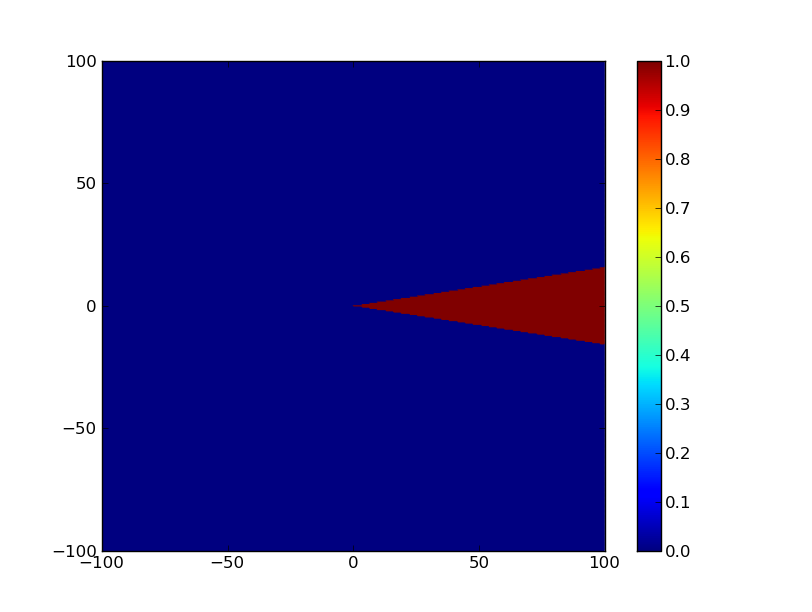
\includegraphics[width=0.48\textwidth]{graphs/sensors/laser.png}
	\end{center}
	\vspace{-30pt}
	\caption{Laser: $\alpha=\frac{\pi}{20}$}
\end{wrapfigure}


\subsection{Distance}
TODO

\begin{figure}
	\vspace{-30pt}
	\begin{center}
		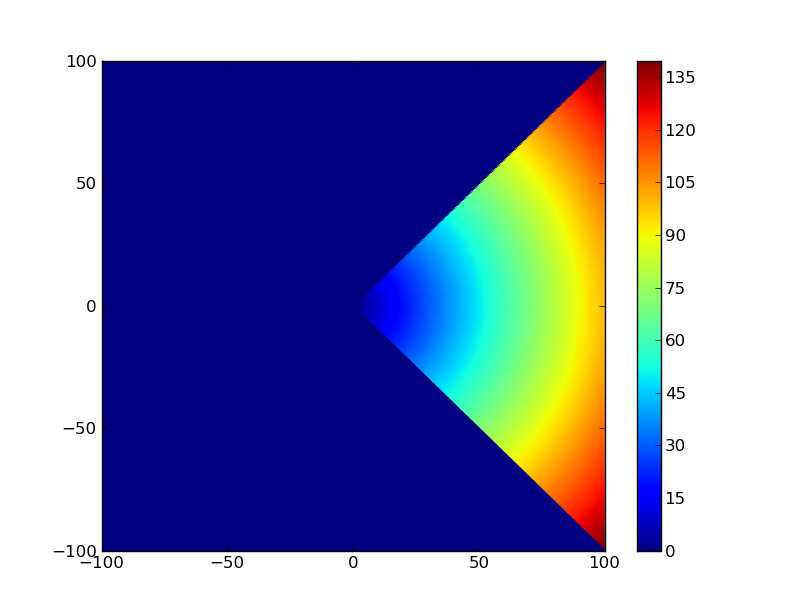
\includegraphics[width=0.48\textwidth]{graphs/sensors/distance.png}
	\end{center}
	\vspace{-30pt}
	\caption{Distance: $\alpha=\frac{\pi}{4}$}
\end{figure}

\subsection{Proximity}
TODO

\begin{wrapfigure}{r}{0.5\textwidth}
	\vspace{-30pt}
	\begin{center}
		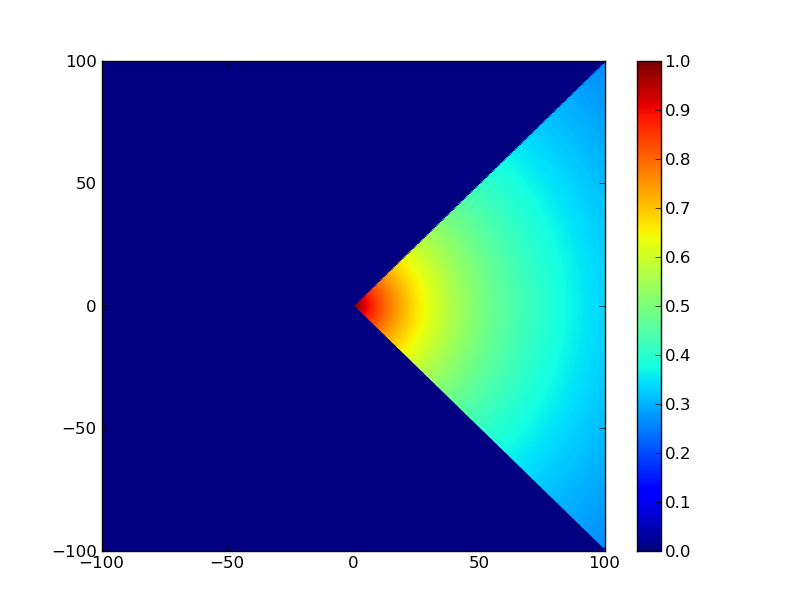
\includegraphics[width=0.48\textwidth]{graphs/sensors/proximity.png}
	\end{center}
	\vspace{-30pt}
	\caption{Proximity: $bias=50$ $\alpha=\frac{\pi}{4}$}
\end{wrapfigure}

\subsection{Smell}
TODO

\begin{wrapfigure}{r}{0.5\textwidth}
	\vspace{-30pt}
	\begin{center}
		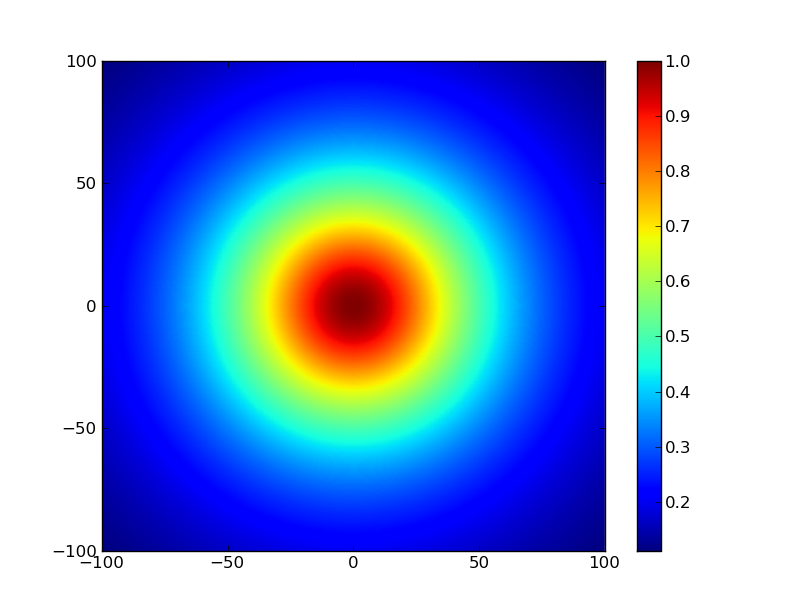
\includegraphics[width=0.48\textwidth]{graphs/sensors/smell.png}
	\end{center}
	\vspace{-30pt}
	\caption{Smell: $bias=50$}
\end{wrapfigure}

\cleardoublepage
\subsection{Light}
\begin{figure}[hb]
	\vspace{-20pt}
	\begin{center}
		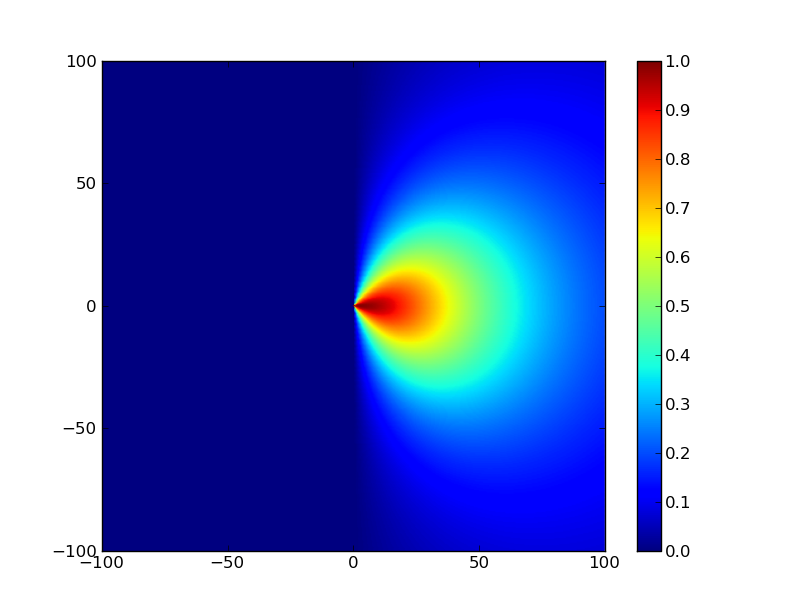
\includegraphics[width=0.6\textwidth]{graphs/sensors/light.png}
	\end{center}
	\vspace{-20pt}
	\caption{Light: $bias=50$ $\alpha=\frac{\pi}{2}$}
\end{figure}

\indent Este sensor permite obter a intensidade de luz captada. Tal como no sensor de cheiro a intensidade transmitida
é comulativa e inversamente proporsional ao quadrado da distância. No entanto este sensor é direcionado (i.e. fontes
directamente á frente do sensor influenciam mais que os existentes na periferia. Assim a intensidade total do sensor é:
\[
	I = \displaystyle\sum\limits_{l \in lights} \frac{l_{i}}{1 + (\frac{l_{d}}{d})^{2}*cos(\frac{2\pi}{\alpha}*l_{\alpha})}
\]

Onde $l_{i}$, $l_{d}$, $l_{\alpha}$ são a intensidade, a distância e o ângulo de visão para cada luz;
$\alpha$ é a abertura do sensor ($rad$);
e $d$ é a distância á qual uma luz com intensidade 1 situada em frente ao sensor produz uma saida no sensor de 0.5.

\cleardoublepage
\subsection{Sound}
\begin{figure}[hb]
	\vspace{-20pt}
	\begin{center}
		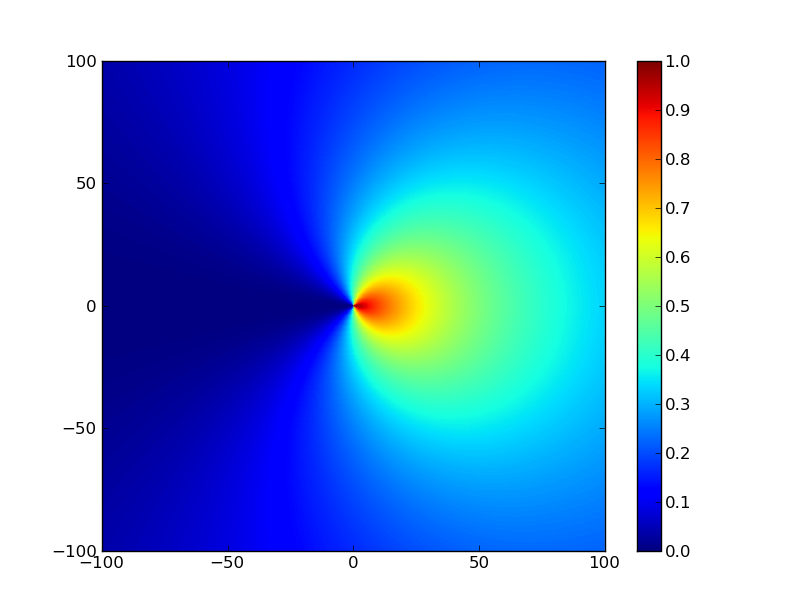
\includegraphics[width=0.6\textwidth]{graphs/sensors/cardioid.png}
	\end{center}
	\vspace{-20pt}
	\caption{Sound: $bias=50$}
\end{figure}

\indent Este sensor indica a intensidade de som captado e pretende simular o
comportamento do ouvido humano. Desta forma fontes de som em frente ao sensor têm mais impacto
mas fontes atrás deste também o influenciam. Este comportamento foi bastante estudado e é aproximado pela função \emph{cardioide} definida em $\theta \in [0..2\pi]$:
\[
	cardioid(\theta) = \frac{1 + cos(\theta)}{2}
\]

\indent Extendendo esta função para 3 dimensões obtemos uma fórmula fechada para a superficie cardioidal
que utilizamos para construir o sensor de som cuja intensidade é
\[
	I = \displaystyle\sum\limits_{s \in sounds}\frac{1+cos(s_{\alpha})}{2}*\frac{s_{i}}{\frac{s_{d}}{d}+1}
\] 

onde $s_{i}$, $s_{d}$, $s_{\alpha}$ são a intensidade, a distância e o ângulo de fonte de som;
e $d$ é a distância à qual uma uma fonte com intensidade 1 situada em frente ao sensor produz uma saída no sensor de 0.5.
Note-se que o resultado deste sensor é semelhante ao do sensor de luz quando $\alpha=\pi$,
mas decresce mais rapidamente quando o ângulo aumenta.

\cleardoublepage
\section{Vehicles}
\subsection{Eight}
\begin{wrapfigure}{r}{0.5\textwidth}
	\begin{center}
		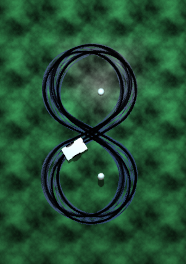
\includegraphics[width=0.48\textwidth]{trail/eight.png}
	\end{center}
	\caption{Trail of the eight vehicle}
\end{wrapfigure}

\begin{wrapfigure}{r}{0.5\textwidth}
	\begin{center}
		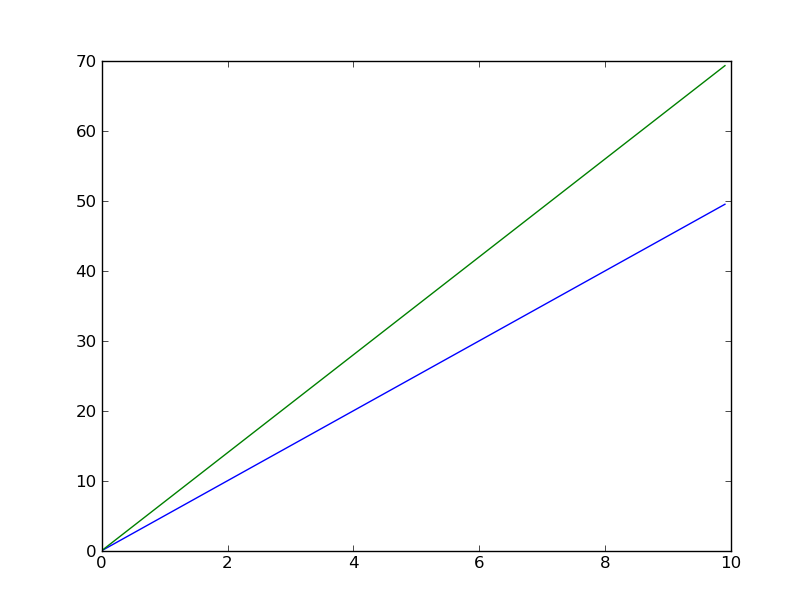
\includegraphics[width=0.48\textwidth]{graphs/activators/eight_l.png}
	\end{center}
	\caption{Left wheel activator functions}
\end{wrapfigure}

\begin{wrapfigure}{r}{0.5\textwidth}
	\begin{center}
		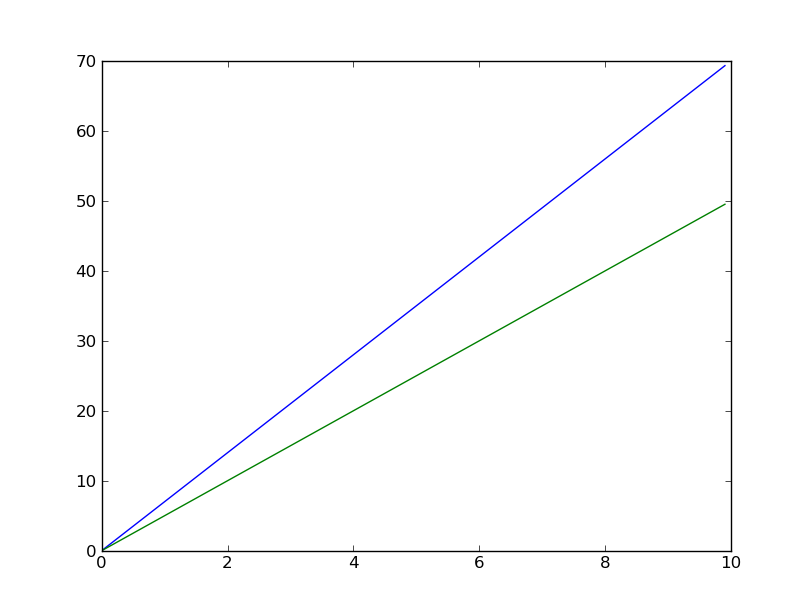
\includegraphics[width=0.48\textwidth]{graphs/activators/eight_r.png}
	\end{center}
	\caption{Right wheel activator functions}
\end{wrapfigure}

\subsection{Ellipse}
\begin{wrapfigure}{r}{0.5\textwidth}
	\begin{center}
		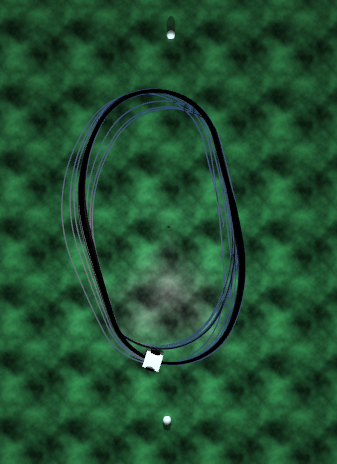
\includegraphics[width=0.48\textwidth]{trail/ellipse.png}
	\end{center}
	\caption{Trail of the ellipse vehicle}
\end{wrapfigure}

\begin{wrapfigure}{r}{0.5\textwidth}
	\begin{center}
		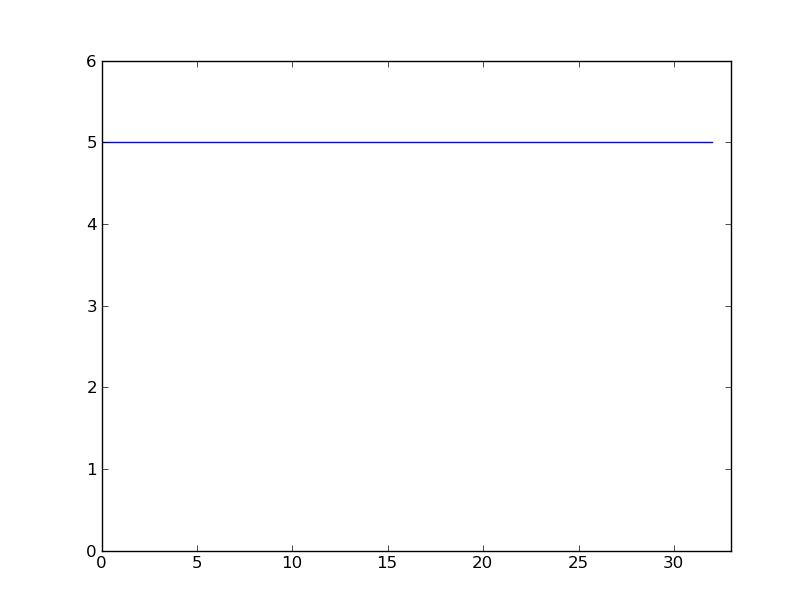
\includegraphics[width=0.48\textwidth]{graphs/activators/ellipse_l.png}
	\end{center}
	\caption{Left wheel activator functions}
\end{wrapfigure}

\begin{wrapfigure}{r}{0.5\textwidth}
	\begin{center}
		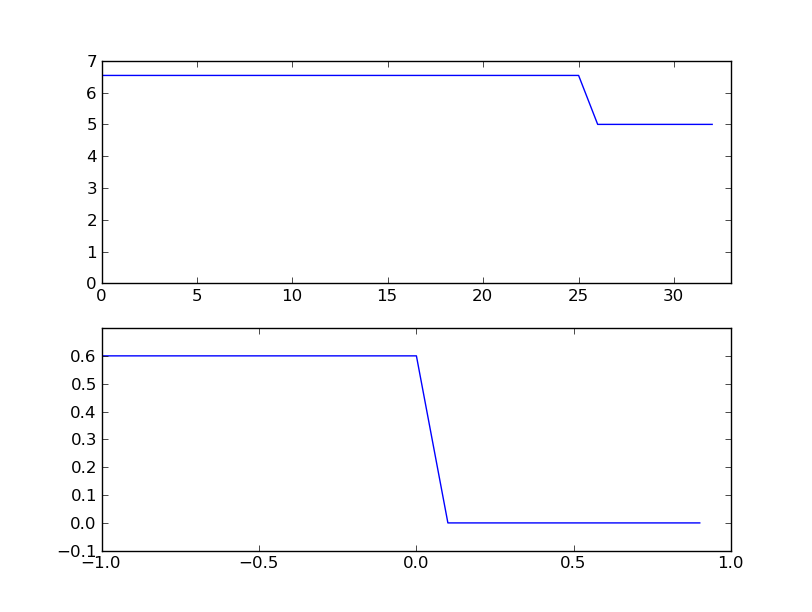
\includegraphics[width=0.48\textwidth]{graphs/activators/ellipse_r.png}
	\end{center}
	\caption{Right wheel activator functions}
\end{wrapfigure}

\subsection{Braitenberg 3c}

\begin{wrapfigure}{r}{0.5\textwidth}
	\begin{center}
		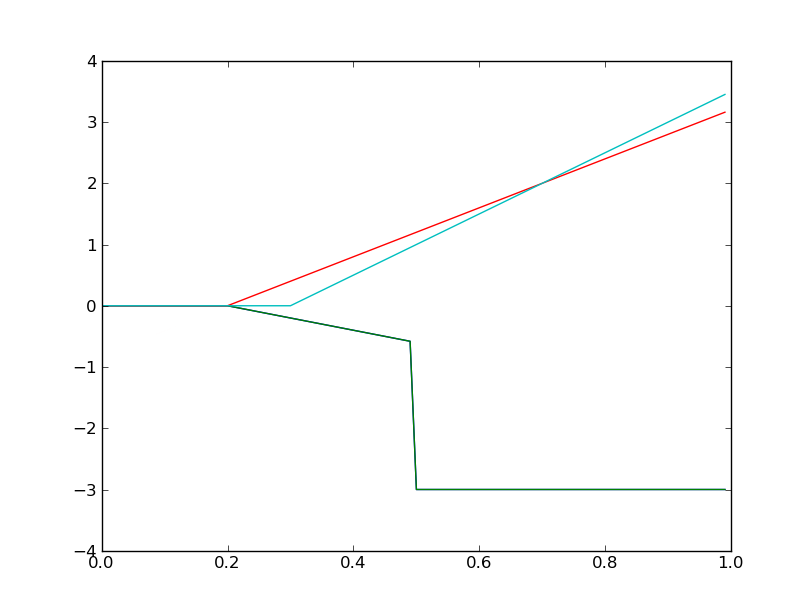
\includegraphics[width=0.48\textwidth]{graphs/activators/3c_l.png}
	\end{center}
	\caption{Left wheel activator functions}
\end{wrapfigure}

\begin{wrapfigure}{r}{0.5\textwidth}
	\begin{center}
		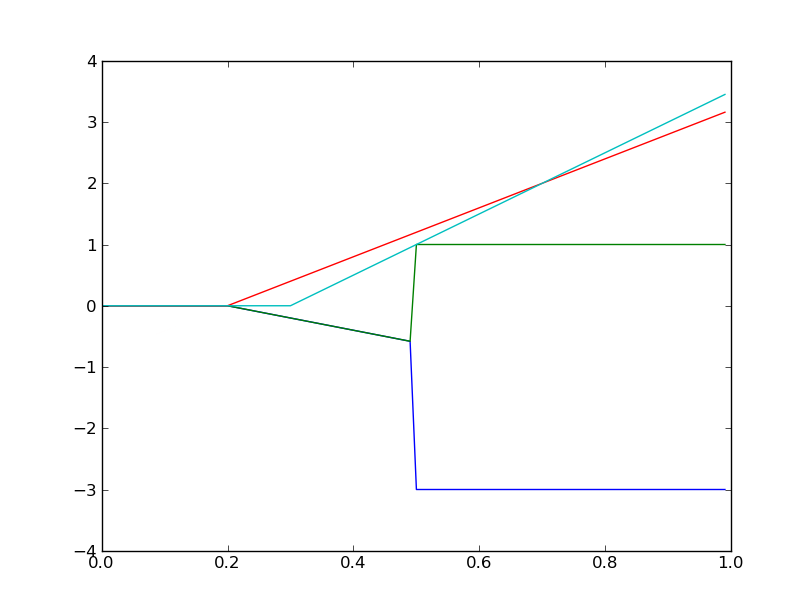
\includegraphics[width=0.48\textwidth]{graphs/activators/3c_r.png}
	\end{center}
	\caption{Right wheel activator functions}
\end{wrapfigure}

\cleardoublepage
\section{Project}


\end{document}
